\chapter{Introduction}
\section{Motivation}
\subsection{Context}
As the robotics industry grows year over year, so does the number of robots operating around the world. It is estimated that there were approximately 3.4 million industrial robots in use worldwide in
2023~\cite{Q0_1_industrial_robots_in_operation}. At the same time, the number of newly installed industrial robots has been increasing steadily since 2014; between 2021 and 2024, around 541\,000 new industrial
robots were installed per year~\cite{Q0_2_industrial_robots_new_installations}. Within this landscape, collaborative robots (cobots) represent about 10.5\% of the industrial robot market, with 57\,040 new units 
deployed in 2023, and annual cobot installations since 2020, 2022, and 2023 reaching roughly 50\,000 units per year; importantly, these cobots are expected to complement rather than replace traditional industrial 
robots~\cite{Q0_3_industrial_robots_new_cobot_installations_BarChart}.

\begin{figure}[ht]
    \centering
    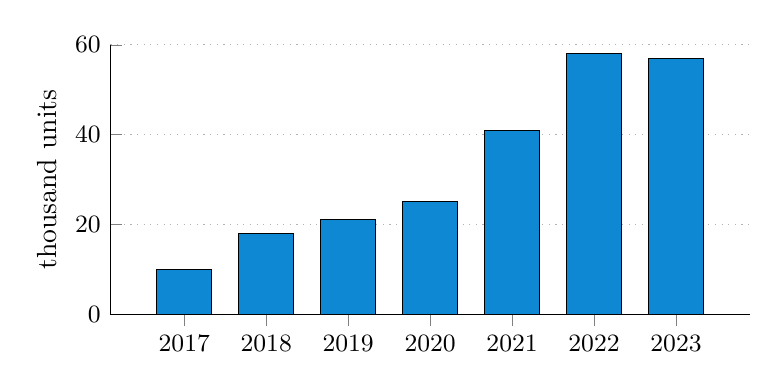
\begin{tikzpicture}
        \begin{axis}[
                ybar,
                bar width=20pt,
                ymin=0, ymax=60,
                width=0.8\linewidth,
                height=5cm,
                enlarge x limits=0.15,
                axis x line*=bottom,
                axis y line*=left,
                ymajorgrids=true,
                grid style={dotted,gray!60},
                ylabel={thousand units},
                xtick=data,
                xticklabels={2017,2018,2019,2020,2021,2022,2023},
                tick label style={font=\small},
            ]
            \addplot[fill=cyan!70!blue] coordinates {
                    (1,10)  % 2017
                    (2,18)  % 2018
                    (3,21)  % 2019
                    (4,25)  % 2020
                    (5,41)  % 2021
                    (6,58)  % 2022
                    (7,57)  % 2023
                };
        \end{axis}
    \end{tikzpicture}
    \caption{Global annual installations of collaborative robots from 2017 to 2023 (in thousand units). Data from~\cite{Q0_3_industrial_robots_new_cobot_installations_BarChart}.}\label{fig:cobot_installations}
\end{figure}

The growing deployment of, and increasing collaboration with, robots imposes stringent requirements on safety and performance. 
As tasks become more complex and humans and robots share workspaces more closely, two closely related problems become central: 
safe manipulation of payloads and safe physical human-robot interaction. 
Addressing both problems requires accurate knowledge of the inertial parameters of the manipulated object together with consistent estimation of the robot's dynamic state and interaction forces. 
A collaborative robot must therefore maintain an internal representation of the mass-inertia properties of the payload or tool it manipulates and of the forces exchanged with its environment. 
This dynamic awareness is a prerequisite for compliant, contact-rich behaviour and for precise, high-performance manipulation in close proximity to humans. HERE NEED TO ADD THE CITES, first sort from old Libaray. (Motivation.md)
